%% ----------------------------------------------------------------
%% Thesis.tex -- MAIN FILE (the one that you compile with LaTeX)
%% ---------------------------------------------------------------- 

% Set up the document
\documentclass[a4paper, 11pt, oneside]{Thesis}  % Use the "Thesis" style, based on the ECS Thesis style by Steve Gunn
\graphicspath{Figures/}  % Location of the graphics files (set up for graphics to be in PDF format)
\usepackage{hyperref}
% Include any extra LaTeX packages required
\usepackage[square, numbers, comma, sort&compress]{natbib}  % Use the "Natbib" style for the references in the Bibliography
\usepackage{verbatim}  % Needed for the "comment" environment to make LaTeX comments
\usepackage{vector}  % Allows "\bvec{}" and "\buvec{}" for "blackboard" style bold vectors in maths
\hypersetup{urlcolor=blue, colorlinks=true}  % Colours hyperlinks in blue, but this can be distracting if there are many links.

%% ----------------------------------------------------------------
\begin{document}
\frontmatter      % Begin Roman style (i, ii, iii, iv...) page numbering

% Set up the Title Page
\title  {The Analysis of Task Scheduling with Unsupervised Self Organizing Map}
\authors  {\texorpdfstring
            {\href{your web site or email address}{Zimo Zhou (xxxxxxx) \\ Uday Singh (xxxxxxx) \\Yaowen Mei (1177855)}}
            {Zimo Zhou, Uday Singh, Yaowen Mei}
            }
\addresses  {\groupname\\\deptname\\\univname}  % Do not change this here, instead these must be set in the "Thesis.cls" file, please look through it instead
\date       {\today}
\subject    {}
\keywords   {}

\maketitle
%% ----------------------------------------------------------------

\setstretch{1.3}  % It is better to have smaller font and larger line spacing than the other way round

% Define the page headers using the FancyHdr package and set up for one-sided printing
\fancyhead{}  % Clears all page headers and footers
\rhead{\thepage}  % Sets the right side header to show the page number
\lhead{}  % Clears the left side page header

\pagestyle{fancy}  % Finally, use the "fancy" page style to implement the FancyHdr headers

%% ----------------------------------------------------------------
\clearpage  % Declaration ended, now start a new page
%% ----------------------------------------------------------------
% The Abstract Page
\addtotoc{Abstract}  % Add the "Abstract" page entry to the Contents
\abstract{
\addtocontents{toc}{\vspace{1em}}  % Add a gap in the Contents, for aesthetics

Dynamic task scheduling is a very famous open question in computer science, it is consisting in generating a task arrangement for scheduling K robots to accomplish M tasks with the minimum possible total traveling length. The same as the famous traveling sales person problem, this is also a NP-Complete problem. This implies that the time requirement for solving this problem increased rapidly as the number of tasks and number of robots increase. Due to this fact, soft computing, especially self organizing map (SOM), could possibly shining a light on finding the optimal or near optimal solution of this problem.  In this paper, different task scheduling algorithms were analysed in terms of accuracy and time efficiency. 
}
\\
\\
\textbf{ Key Words}: SOM, Algorithms, NP-Complete, Soft Computing

\clearpage  % Abstract ended, start a new page
%% ----------------------------------------------------------------
%% ----------------------------------------------------------------

\pagestyle{fancy}  %The page style headers have been "empty" all this time, now use the "fancy" headers as defined before to bring them back


%% ----------------------------------------------------------------
\lhead{\emph{Contents}}  % Set the left side page header to "Contents"
\tableofcontents  % Write out the Table of Contents

%% ----------------------------------------------------------------
\lhead{\emph{List of Figures}}  % Set the left side page header to "List if Figures"
\listoffigures  % Write out the List of Figures

%% ----------------------------------------------------------------
\lhead{\emph{List of Tables}}  % Set the left side page header to "List of Tables"
\listoftables  % Write out the List of Tables

%% ----------------------------------------------------------------
\setstretch{1.5}  % Set the line spacing to 1.5, this makes the following tables easier to read
\clearpage  % Start a new page
%% ----------------------------------------------------------------
% % End of the pre-able, contents and lists of things
% % Begin the Dedication page

% \setstretch{1.3}  % Return the line spacing back to 1.3

% \pagestyle{empty}  % Page style needs to be empty for this page
% \dedicatory{For/Dedicated to/To my\ldots}

% \addtocontents{toc}{\vspace{2em}}  % Add a gap in the Contents, for aesthetics


%% ----------------------------------------------------------------
\mainmatter	  % Begin normal, numeric (1,2,3...) page numbering
\pagestyle{fancy}  % Return the page headers back to the "fancy" style

% Include the chapters of the thesis, as separate files
% Just uncomment the lines as you write the chapters
\lhead{}  % remove header
\chapter{Introduction of the Task Scheduling Problem}
In modern era, with the development of artificial intelligent and machine learning technology, robots are becoming deeply integrated into people's life. Therefore, robot path planning is a hot topic that attacks a lot of scientists attention. Among all these robot path planning problems, due to the wide potential of application, \textbf{task scheduling} is one of the most famous question that that has been under debate for long time. There are many versions of problem statement for this task scheduling problem, but one of the most basic and fundamental format is stated as the following: 
\section{Problem Statement}
Assume there are K homogeneous robots and M targets randomly distributed in a bounded 2D space. Each target requires \textbf{at least one} robot, and each of the robots need to be assigned to one target (in this basic format, we are not considering the situation where one robot can do multiply tasks). This is to say, the task assignment, $f$ , is a map on $\mathbf{R^2}$ from set $\mathbf{Robots}$ to set $\mathbf{Tasks}$. 
\begin{equation}
    f:{\mathbf{Robots}} \to \mathbf{Tasks}
\end{equation}
The cost function, $C$, is defined as the summation of robots' travelling path from their origin to their assigned tasks:
\begin{equation}
   C = \sum\limits_{{\rm{robots}}} {{\rm{Path\quad } \rm{Length}}} 
\end{equation}
\\
The challenge is to develop a good algorithm to find a traveling path for all the robots with the minimum or near minimal cost.
\\
A visual illustration is given as shown in the picture \ref{fig:birds}, all the M green squares are tasks (in this case, $M=5$, and tasks are labeled as $T_0$ to $T_4$) need to be accomplished, and all the K red dots are robots (in this case, $K=8$, and robots are labeled as $R_0$ to $R_8$) that need to be assigned for a task. All the initial position for tasks and robots are randomly generated in the range of $[0,5]$, and the arrangement with the lowest cost is la-bled with red lines which are generate from a \href{https://github.com/ENGG6570/Group-Project/tree/main/ENGG6570_Project}{Python brute-force program}  . 

\begin{figure}[h!]
  \centering
  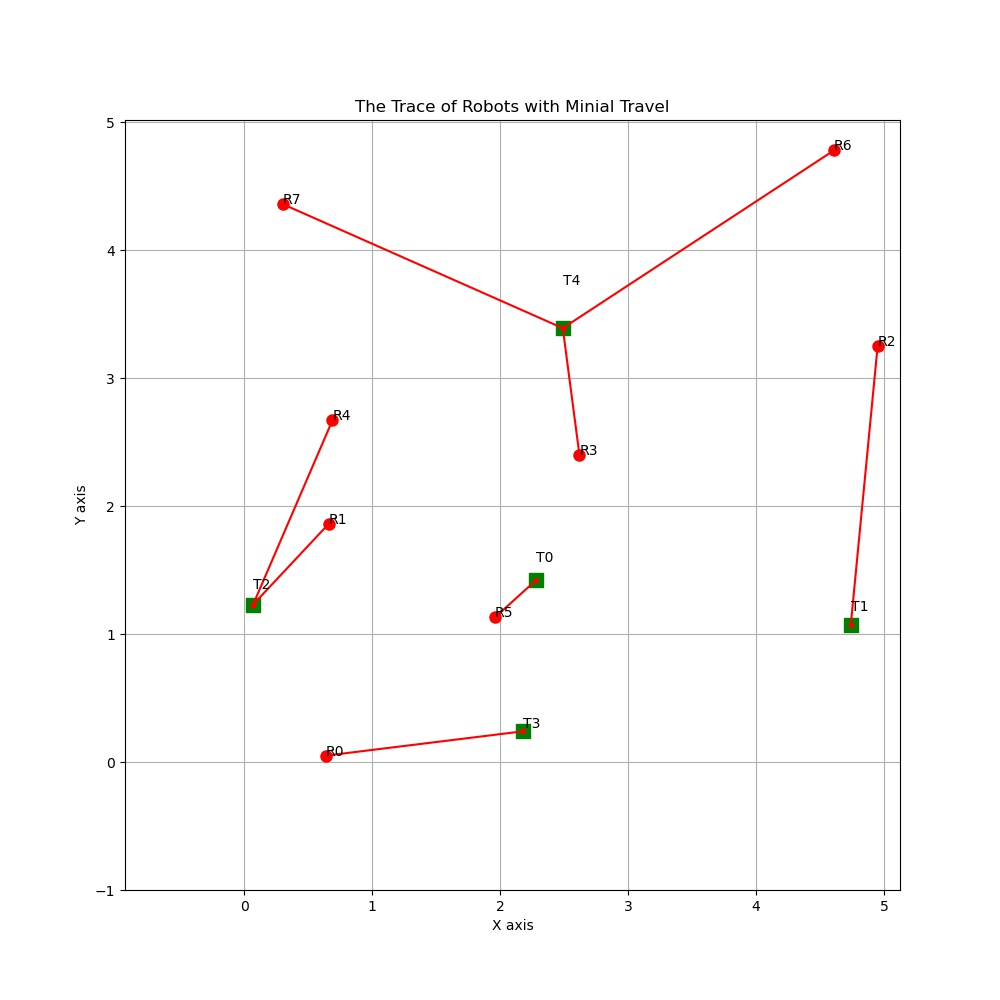
\includegraphics[width=15cm]{Pictures/ProblemStatement.jpeg}
  \caption{The illustration of Task Scheduling Problem with 5 tasks and 8 robots.}
  \label{fig:birds}
  \Description{}
\end{figure}

\section{The Brute-force Method}
Theoretically, at small scale, we can solve this problem and find the best solution with the Brute-force method. The time complexity will be bound by $O(M^K)$. Same as the famous traveling sales person (TSP) problem, this is a NP-complete problem as well.
\subsection{Entropy of this problem}
\\ According to Shannon's information theory\cite{Shannon1948}, for a random variable $X$ in a finite set $\chi$ with probability distribution $p(x)$ , the  Shannon's entropy can be written as:
\begin{equation}
    H\left( X \right) =  - \sum\limits_{x \in \chi } {p\left( x \right){{\log }_2}\left( {p\left( x \right)} \right)}\label{shannon}
\end{equation}
For each of the robots, it will have at most M choice to choose from as its the target. The total number of possible of arrangement is at most $M^K$. With considering the boundary condition that each of these M target need to have at least one robot, we can reduce the total number of possible of arrangement, $\chi$, as: 

\begin{equation}
\begin{array}{*{20}{c}}
\chi & = &{\underbrace {M\left( {M - 1} \right)\left( {M - 2} \right) \ldots 1}_{M!} \times C_{K - M}^K{M^{K - M}}}\\
{}& = &{M!\frac{{K!}}{{\left( {K - K + M} \right)!\left( {K - M} \right)!}}{M^{K - M}}}\\
{}& = &{\frac{{K!}}{{\left( {K - M} \right)!}}{M^{K - M}}}
\end{array}
\end{equation}

\subsection{Time Analysis and Entropy Analysis}
With a home used i7-9700K CPU (8 Cores, 3.6GHz), the maximum scale size of this problem that can be solved without memory leaking is 2 tasks and 20 robots (See Figure \ref{fig:upperlimit}), or, 8 robots and 8 tasks. Table \ref{tab:bruteforce} is a summaries the time complexity of this problem with the Brute-force method:

\begin{table}[]
    \centering
\begin{tabular}{|l|l|l|l|l|}
\hline
M & K  & Time     & $\chi$       & $H(\chi)$ \\ \hline
2 & 2  & 0.0005   & 2       &  1.000 \\ \hline
2 & 4  & 0.0005   & 14      &  3.807 \\ \hline
2 & 8  & 0.001488 & 254     &  7.988 \\ \hline
2 & 16 & 0.65571  & 65534   &  15.999 \\ \hline
2 & 20 & 13.02    & 1048574 &   20.000\\ \hline
\end{tabular}
    \caption{The time complexity analysis of this problem with 2 tasks, and $K = 2^n$ robots}
    \label{tab:bruteforce}
\end{table}

\begin{figure}[h!]
  \centering
  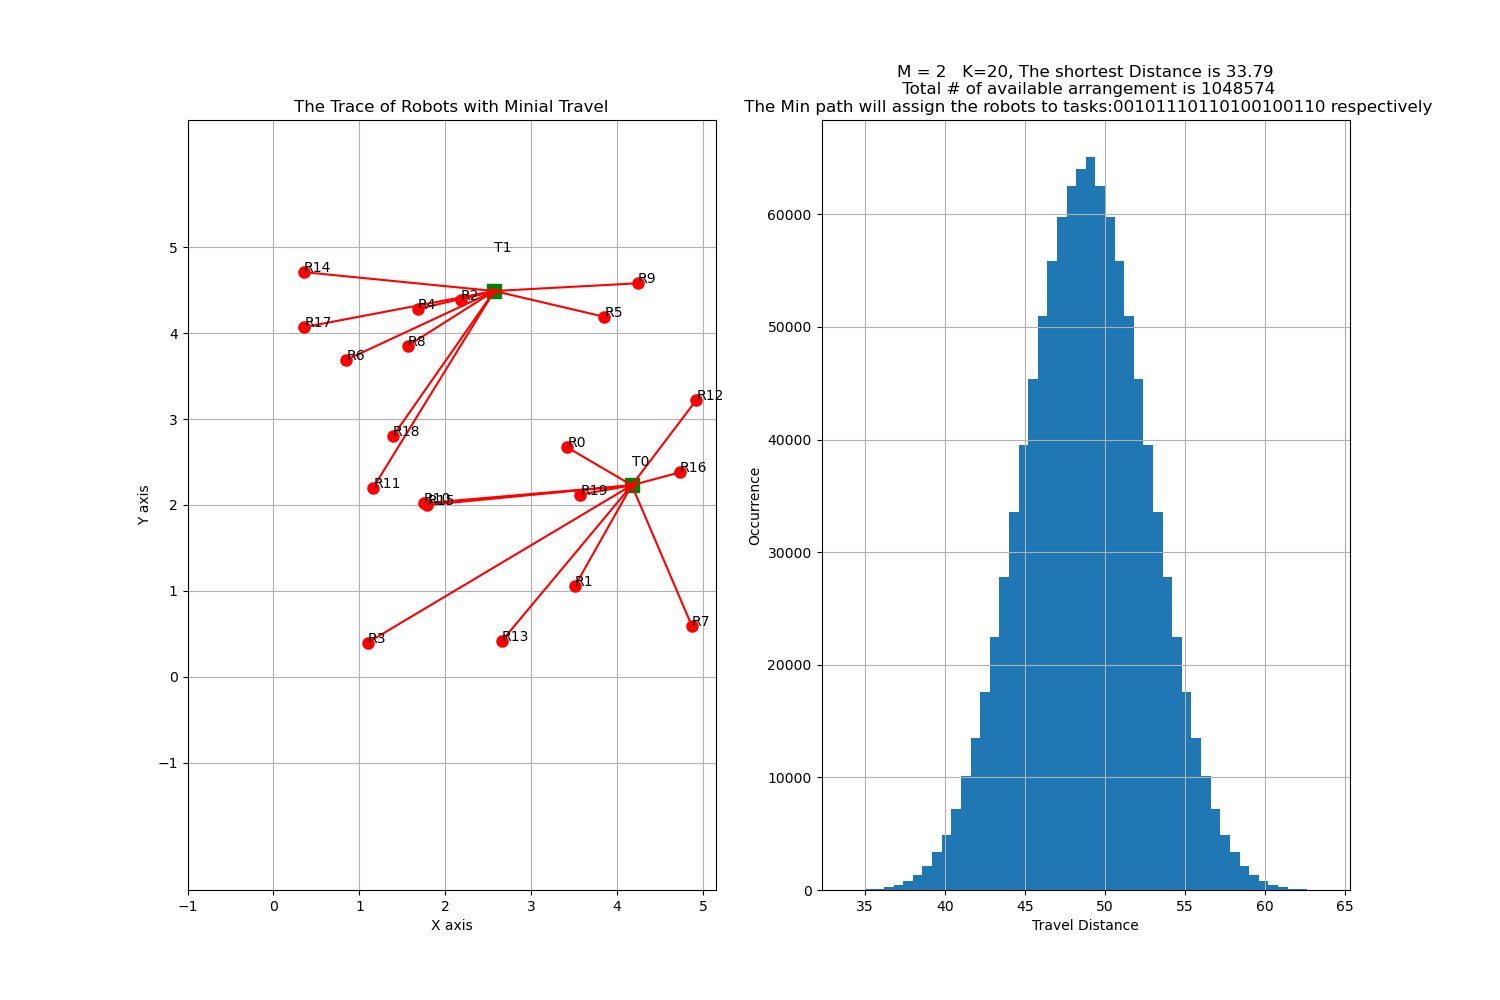
\includegraphics[width=15cm]{Pictures/220.png}
  \caption{The maximum scale size of this problem that can be solved on a PC is 2 tasks and 20 robots}
  \label{fig:upperlimit}
  \Description{}
\end{figure} % Introduction

\chapter{Overview of the Previous Work}

\section{The history of Self Organizing Map (SOM)}
Self-Organizing Map (SOM), also know as Kohonen map, is a topological preserving map that can map a higher dimensional space to a lower dimensional space. Along this process, information will be compressed; while, the key parameters in terms of "topological and metric relationships"\cite{Kohonen1998} will be retained. 
\\
There are two steps involved in forming a self-organizing map from a raw input data-set\cite{hebbian2007}, respectively to be 1) \textbf{competition} and 2) \textbf{cooperation}. When a set of data is feed into the system sequentially with random shuffle, for each input data point, \textbf{competition} will take place first and, based on a pre-defined cost function, one of the neurons on the output layer with the minimal cost will be selected as a winner; Following the competition, the  \textbf{cooperation} will then take place. Based on a neighbourhood function, the winner together with it's neighbour neurons will proceed the learning; while, the neurons outside of the winner's neighbour zone will gain no learning. The purpose of the cooperation step is to increase the like-hood that if a similar input pattern present again, the same group of neurons will become the winner with a higher possibility. Iterate with this strategy on the input data-set over a suitable period, without supervising (providing error to the system), the output layer will simultaneously form a map that contains the similar topological structure as the input data. 

\section{Solving the task scheduling problem with SOM }
\subsection{Task scheduling with K output neurons}
In 2006, based on the SOM approach, Anmin and Simon proposed a new method to solve the multi-robot system problems in a multi-agent architecture\cite{zhu2006k}. In this research, robots are scheduled to approach the targets by competition and cooperation. 
\\
The robots and targets are assumed to be randomly initialized in a bounded area. Conventional method are limited with the restriction that all the targets are static. However, in this algorithm proposed by Anmin, the path planning and robots’ movements start synchronously. The left panel in Figure \ref{fig-2} shows the model of this architecture: there are 2 neurons on the input layer and K neurons on the output layer that are representing the coordinate locations of the target and the coordinate locations of the K robots, respectively. The K connecting weight vectors, $\{w_jx , w_jy\}$, where j = 1, 2, …, K, are computed from the Euclid distance between the input task and the location of each of the robots. In each epoch, the robot with the lowest distance is selected as the winner and the weight vectors within the winner’s neighbourhood zone will be updated to approaching the input target. All the targets will be input to the model in a random sequence in each iteration.

\begin{figure}[h]
  \centering
  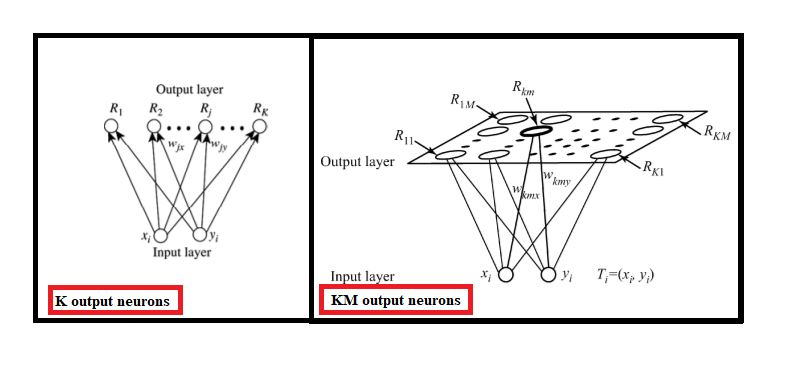
\includegraphics[width=15cm]{Pictures/SimonAmin2Methods.JPG}
  \caption{The illustration of two SOM configuration\cite{zhu2006neural,zhu2006k}.}
  
  \Description{The figure on the left has $K$ neurons on the output layer\cite{zhu2006k}; while, the figure on the right has $KM$ neurons on the output layer\cite{zhu2006neural}}
  \label{fig-2}
\end{figure}

Another interesting idea in this paper is the path planning for multi-robot systems. Several depots randomly distribute in the area. The task for robots is to get the goods from depots and reach the destination in the end. Thus, K M nodes are used in this task. Each robot has a group of M neuron to do the planning of K paths for robots. Here, each neurons used a term P to control the workload for each robot. The distance computation is multiplied by the term P, which is regards as:

\begin{equation}
    P = \frac{{L + V}}{{1 + V}}
\end{equation}

Where, L represent the path of the robot and V is the average path length. 
\subsection{Task Scheduling with KM output neurons}
As illustrating on the right panel of Figure \ref{fig-2}, Anmin had also proposed a different method to solve this problem. In the second paper\cite{zhu2006neural}, the K M neurons are used in the second layer of self-organizing map to do the path planning for dynamic task. For path planning problems, the M neurons are assigned to a group for K robots. Also, the P control is also used to balance the workload for K robots as the previous paper. By doing this, the dynamic trajectories can be recorded with workload balance.  In this task, the targets move a step in a random direction in each iteration. And the robot can still get to the target successfully. Although the path is not a near-optimal solution for the task, the task can be completed in computational time.  % Overview of the Previous W

\chapter{The Proposed Approach to the Problem}
In this section, you should briefly outline your work for this problem: what do you
plan to do in your project? What results may you expect to have? You don't need to
give any details of your approach in your proposal, just list the ideas you plan to use to
solve the problems. Of course, if you know some details, you can put them here, e.g.,
your preliminary results. When you write your interim report, you should provide the
details of your proposed approach. % The Proposed Approach to the Problem

% \chapter{Results} % Results

\chapter{Discussion}
In this section, you may present your preliminary ideas on how your work can be
compared with previous works or related works: what's new for your work? What are
the differences of your work from existing works? What the advantages and
limitations of your approach? How the parameter variation in your model may result
the model performance (parameter sensitivity of your model)? How would you
improve you work in the future (beyond this course project)? … % Discussion

\chapter{Summary}
In this section, conclude what have in this proposal, and summarize the important
points naturally drawn from the proposal.  % Summary

%\input{Chapters/Chapter7} % Conclusion

%% ----------------------------------------------------------------
% Now begin the Appendices, including them as separate files

% \addtocontents{toc}{\vspace{2em}} % Add a gap in the Contents, for aesthetics

% \appendix % Cue to tell LaTeX that the following 'chapters' are Appendices

% \chapter{An Appendix}

Lorem ipsum dolor sit amet, consectetur adipiscing elit. Vivamus at pulvinar nisi. Phasellus hendrerit, diam placerat interdum iaculis, mauris justo cursus risus, in viverra purus eros at ligula. Ut metus justo, consequat a tristique posuere, laoreet nec nibh. Etiam et scelerisque mauris. Phasellus vel massa magna. Ut non neque id tortor pharetra bibendum vitae sit amet nisi. Duis nec quam quam, sed euismod justo. Pellentesque eu tellus vitae ante tempus malesuada. Nunc accumsan, quam in congue consequat, lectus lectus dapibus erat, id aliquet urna neque at massa. Nulla facilisi. Morbi ullamcorper eleifend posuere. Donec libero leo, faucibus nec bibendum at, mattis et urna. Proin consectetur, nunc ut imperdiet lobortis, magna neque tincidunt lectus, id iaculis nisi justo id nibh. Pellentesque vel sem in erat vulputate faucibus molestie ut lorem.

Quisque tristique urna in lorem laoreet at laoreet quam congue. Donec dolor turpis, blandit non imperdiet aliquet, blandit et felis. In lorem nisi, pretium sit amet vestibulum sed, tempus et sem. Proin non ante turpis. Nulla imperdiet fringilla convallis. Vivamus vel bibendum nisl. Pellentesque justo lectus, molestie vel luctus sed, lobortis in libero. Nulla facilisi. Aliquam erat volutpat. Suspendisse vitae nunc nunc. Sed aliquet est suscipit sapien rhoncus non adipiscing nibh consequat. Aliquam metus urna, faucibus eu vulputate non, luctus eu justo.

Donec urna leo, vulputate vitae porta eu, vehicula blandit libero. Phasellus eget massa et leo condimentum mollis. Nullam molestie, justo at pellentesque vulputate, sapien velit ornare diam, nec gravida lacus augue non diam. Integer mattis lacus id libero ultrices sit amet mollis neque molestie. Integer ut leo eget mi volutpat congue. Vivamus sodales, turpis id venenatis placerat, tellus purus adipiscing magna, eu aliquam nibh dolor id nibh. Pellentesque habitant morbi tristique senectus et netus et malesuada fames ac turpis egestas. Sed cursus convallis quam nec vehicula. Sed vulputate neque eget odio fringilla ac sodales urna feugiat.

Phasellus nisi quam, volutpat non ullamcorper eget, congue fringilla leo. Cras et erat et nibh placerat commodo id ornare est. Nulla facilisi. Aenean pulvinar scelerisque eros eget interdum. Nunc pulvinar magna ut felis varius in hendrerit dolor accumsan. Nunc pellentesque magna quis magna bibendum non laoreet erat tincidunt. Nulla facilisi.

Duis eget massa sem, gravida interdum ipsum. Nulla nunc nisl, hendrerit sit amet commodo vel, varius id tellus. Lorem ipsum dolor sit amet, consectetur adipiscing elit. Nunc ac dolor est. Suspendisse ultrices tincidunt metus eget accumsan. Nullam facilisis, justo vitae convallis sollicitudin, eros augue malesuada metus, nec sagittis diam nibh ut sapien. Duis blandit lectus vitae lorem aliquam nec euismod nisi volutpat. Vestibulum ornare dictum tortor, at faucibus justo tempor non. Nulla facilisi. Cras non massa nunc, eget euismod purus. Nunc metus ipsum, euismod a consectetur vel, hendrerit nec nunc.	% Appendix Title

%\input{Appendices/AppendixB} % Appendix Title

%\input{Appendices/AppendixC} % Appendix Title

% \addtocontents{toc}{\vspace{2em}}  % Add a gap in the Contents, for aesthetics
% \backmatter

%% ----------------------------------------------------------------
\label{Bibliography}
\lhead{\emph{Bibliography}}  % Change the left side page header to "Bibliography"
\bibliographystyle{unsrtnat}  % Use the "unsrtnat" BibTeX style for formatting the Bibliography
\bibliography{Bibliography}  % The references (bibliography) information are stored in the file named "Bibliography.bib"

\end{document}  % The End
%% ----------------------------------------------------------------